% ============================================================
% How Much ML Code Similarity Is Framework-Dictated?
% Measuring Accidental Clone Prevalence in PyTorch Projects
%
% For submission to Empirical Software Engineering (EMSE)
% Uses article class; swap to svjour3 for final Springer submission
% ============================================================

\documentclass[11pt,a4paper]{article}

% --- Packages ---
\usepackage[utf8]{inputenc}
\usepackage[T1]{fontenc}
\usepackage{lmodern}
\usepackage[margin=2.5cm]{geometry}
\usepackage{graphicx}
\usepackage{booktabs}
\usepackage{tabularx}
\usepackage{amsmath}
\usepackage{hyperref}
\usepackage{xcolor}
\usepackage{enumitem}
\usepackage{float}
\usepackage{caption}
\usepackage{subcaption}
\usepackage{natbib}
\usepackage{url}
\usepackage{listings}
\usepackage{setspace}

\onehalfspacing

\hypersetup{
    colorlinks=true,
    linkcolor=blue!60!black,
    citecolor=blue!60!black,
    urlcolor=blue!60!black,
}

\lstset{
    basicstyle=\ttfamily\small,
    breaklines=true,
    frame=single,
    language=Python,
    showstringspaces=false,
}

% --- Placeholder command for future data ---
\newcommand{\placeholder}[1]{\textbf{[#1]}}

% ============================================================
\begin{document}

\title{How Much ML Code Similarity Is Framework-Dictated?\\
Measuring Accidental Clone Prevalence in PyTorch Projects}

\author{Joseph C.\ Sremack\\
Resolution Economics\\
\texttt{jsremack@gmail.com}}

\date{}
\maketitle

% ============================================================
\begin{abstract}
Code similarity measurement underpins clone detection, plagiarism identification, and software intellectual property analysis. Machine learning frameworks such as PyTorch impose rigid structural conventions (training loops, model definitions, data loading patterns) that cause independently developed projects to converge on nearly identical code. This framework-driven similarity produces \emph{accidental clones}: detected similarities that reflect shared API constraints rather than copying. Despite growing reliance on code similarity tools in ML software contexts, no empirical study has measured what proportion of ML project code is framework-dictated or how filtering such boilerplate affects measured similarity between independent projects.

We present an empirical study of 15 verified-independent PyTorch projects spanning five ML domains (computer vision, NLP, audio, generative modeling, and other). We develop an AST-based classifier that categorizes every function and class as framework boilerplate, API protocol code, or custom implementation, validated against PyTorch's official documentation and through intra-rater reliability assessment. We apply JPlag clone detection to all pairwise project combinations before and after filtering framework-dictated code, measuring the \emph{filtration effect}, the change in similarity attributable to shared boilerplate. Sensitivity analyses across multiple classification and detection thresholds assess the robustness of findings. This study contributes the first empirical baseline for accidental clone prevalence in ML framework code and a reusable methodology for boilerplate-aware similarity measurement.
\end{abstract}

\noindent\textbf{Keywords:} code clones, boilerplate code, machine learning, PyTorch, code similarity, software forensics

% ============================================================
\section{Introduction}
\label{sec:intro}

Code similarity measurement is foundational to software engineering research and practice. Clone detection tools identify duplicated code to support maintenance and refactoring. Plagiarism detectors flag unauthorized reuse in educational and commercial settings. In forensic software analysis, pairwise similarity scores inform legal judgments about whether one codebase was derived from another. Across all of these applications, the core assumption is that high measured similarity between two codebases indicates a meaningful relationship between them: that one was copied from, influenced by, or derived from the other.

This assumption breaks down when independently developed programs share a common framework. Juergens, Deissenboeck, and Hummel~\citep{juergens2010} introduced the concept of \emph{accidental clones}, code similarities arising from shared API constraints rather than copying. In their controlled experiment, 109 students independently implemented the same specification without a shared framework, and clone detection rates were below 1\%. Their finding established an important baseline: when developers work independently without shared structural constraints, detected similarity is negligible.

The landscape of modern software development, however, has shifted dramatically since that baseline was established. Machine learning frameworks such as PyTorch, TensorFlow, and Hugging Face Transformers impose rigid structural conventions on the code that uses them. A PyTorch training loop, for example, follows a mandatory sequence: \texttt{optimizer.zero\_grad()}, forward pass, loss computation, \texttt{loss.backward()}, \texttt{optimizer.step()}, which appears in virtually identical form across every project that trains a neural network. Model definitions must inherit from \texttt{nn.Module} and implement \texttt{\_\_init\_\_} and \texttt{forward} methods. Data loading requires \texttt{Dataset} subclasses with \texttt{\_\_len\_\_} and \texttt{\_\_getitem\_\_}. These are not stylistic choices; they are constraints imposed by the framework's API design.

Recent empirical studies confirm that this structural convergence is pervasive. Sens et al.~\citep{sens2025} analyzed 2,928 ML systems and found that 58\% contain duplicated model implementation files. Nahar et al.~\citep{nahar2025} studied 262 ML products and found shared architectural patterns across independently developed products. Yet neither study measured \emph{how much} of this convergence is framework-dictated versus reflecting genuine design similarity.

This gap has practical consequences. Code similarity tools, when applied to ML projects without accounting for framework boilerplate, will report inflated similarity scores between projects that share no meaningful relationship. Ragkhitwetsagul, Krinke, and Clark~\citep{ragkhitwetsagul2018} demonstrated this problem empirically: in their comparison of 30 similarity analysis tools, boilerplate code was an explicit experimental scenario that confounded tool accuracy. They showed that the problem exists but did not measure its magnitude in real ML projects.

Despite this clear gap, no empirical study has measured what proportion of ML framework code is framework-dictated, or quantified how filtering such boilerplate changes measured similarity between independent projects. This paper addresses that gap with four research questions:

\begin{description}[leftmargin=1cm]
\item[RQ1:] What proportion of code in independent PyTorch ML projects is classifiable as framework boilerplate versus custom implementation?
\item[RQ2:] What is the baseline pairwise code similarity between verified-independent PyTorch projects sharing the same ML domain?
\item[RQ3:] How much does filtering framework boilerplate change measured similarity between independent projects?
\item[RQ4:] Are these measurements stable across classification thresholds?
\end{description}

To answer these questions, we present an empirical study of 15 verified-independent PyTorch projects spanning five ML domains: computer vision, natural language processing, audio, generative modeling, and other. We develop an AST-based classifier that categorizes every function, method, and class as one of three types: \emph{framework boilerplate} (code whose structure is dictated by PyTorch's API), \emph{API protocol code} (code that follows framework conventions with domain-specific configuration), or \emph{custom implementation} (code reflecting developer-specific design choices). The classifier is validated against PyTorch's official documentation as ground truth and through an intra-rater reliability assessment.

We apply JPlag, a well-established token-based similarity detector~\citep{jplag2000}, to all pairwise project combinations in two conditions: using full project code and using custom-only code after filtering boilerplate. The difference between these two measurements (which we term the \emph{filtration effect}) quantifies how much measured similarity is attributable to shared framework code rather than meaningful design similarity.

This study makes four contributions:

\begin{enumerate}
\item An AST-based classification methodology that operationalizes Kapser and Godfrey's~\citep{kapser2008} clone taxonomy for ML framework code, validated against framework documentation.
\item The first empirical measurement of boilerplate prevalence across independent PyTorch projects, providing baselines that were previously unavailable.
\item A measured \emph{filtration effect} showing how much code similarity analysis changes after accounting for framework-dictated code, the novel measurement no prior study has reported.
\item A replication package including the validated classifier, classification manifests, and all analysis scripts, enabling reproduction and extension to other frameworks.
\end{enumerate}

The remainder of this paper is organized as follows. Section~\ref{sec:related} reviews related work. Section~\ref{sec:method} describes our study design. Section~\ref{sec:results} presents results. Section~\ref{sec:discussion} discusses findings and implications. Section~\ref{sec:threats} addresses threats to validity. Section~\ref{sec:conclusion} concludes.


% ============================================================
\section{Background and Related Work}
\label{sec:related}

\subsection{Code Clones and Clone Detection}

Code clones, segments of code that are similar or identical to each other, have been extensively studied in software engineering. Roy, Cordy, and Koschke~\citep{roy2009} provide a comprehensive comparison of detection techniques, categorizing approaches as text-based, token-based, AST-based, PDG-based, and metrics-based. The standard taxonomy distinguishes four clone types: Type-1 (exact copies), Type-2 (syntactically identical with variable renaming), Type-3 (near-miss clones with modifications), and Type-4 (semantically similar but syntactically different)~\citep{roy2007survey}.

Clone detection tools vary in their approach and sensitivity. NiCad~\citep{cordy2011} uses AST-based comparison via TXL transformation, detecting Type-1 through Type-3 clones with configurable thresholds. JPlag~\citep{jplag2000} uses token-based comparison, originally designed for plagiarism detection in educational settings. Ain et al.~\citep{ain2019} provide a recent systematic review cataloguing 97 clone detection tools. Svajlenko and Roy~\citep{svajlenko2015} introduced BigCloneBench, a large-scale benchmark for evaluating clone detection tools against ground truth.

\subsection{Accidental Clones and Boilerplate}

Not all detected clones represent meaningful copying. Juergens, Deissenboeck, and Hummel~\citep{juergens2010} formalized the concept of \emph{accidental clones}, defined as code similarities that arise from shared API constraints, language idioms, or specification requirements rather than from one developer copying another's code. In their experiment, 109 students independently implemented the same specification without access to each other's code or a shared framework. Clone detection rates were below 1\%, establishing a baseline for similarity that arises from shared task requirements alone.

Kapser and Godfrey~\citep{kapser2008} developed a taxonomy of clone patterns that includes boilerplate clones, API protocol clones, and language idioms, arguing that many clones are unavoidable or even beneficial. Their taxonomy provides the conceptual foundation for our classification scheme: our Category~A (framework boilerplate) corresponds to their boilerplate pattern, Category~B (API protocol) to their API protocol pattern, and Category~C (custom implementation) to code that would not appear as a clone pattern in their taxonomy.

Ragkhitwetsagul, Krinke, and Clark~\citep{ragkhitwetsagul2018} tested 30 code similarity analysis tools across multiple scenarios, including a boilerplate injection scenario. They demonstrated that boilerplate code confounds similarity tools by inflating measured similarity, but they did not measure boilerplate prevalence in real-world ML projects. Our study fills this gap by measuring both prevalence and its effect on similarity scores.

\subsection{ML Software Engineering}

Machine learning software has distinctive characteristics that affect code similarity analysis. Sens et al.~\citep{sens2025} analyzed the structure of 2,928 ML systems, finding that 58\% contain duplicated model implementation files. Their work documents the prevalence of duplication but does not distinguish framework-dictated duplication from meaningful reuse. Nahar et al.~\citep{nahar2025} studied 262 ML products and found that independently developed products converge on shared architectural patterns. This convergence is consistent with the framework effect we hypothesize: when developers use the same ML framework, their code necessarily shares structural patterns.

\subsection{Gap}

Prior work establishes that (1)~accidental clones exist and arise from shared constraints, but this was measured without a shared framework~\citep{juergens2010}; (2)~boilerplate and API protocol clones are recognized categories~\citep{kapser2008}, but their prevalence in ML code is unknown; (3)~boilerplate confounds similarity tools~\citep{ragkhitwetsagul2018}, but the magnitude of this confound in ML projects has not been measured; and (4)~ML code exhibits high duplication~\citep{sens2025} and structural convergence~\citep{nahar2025}, but the framework-driven component has not been isolated. Our study provides the first empirical measurement of framework-driven code similarity in ML projects and quantifies the effect of filtering it out.


% ============================================================
\section{Study Design}
\label{sec:method}

Figure~\ref{fig:pipeline} provides an overview of the study pipeline. The study has four phases: data collection, AST-based classification, similarity measurement, and analysis.

\begin{figure}[t]
\centering
\fbox{\parbox{0.9\textwidth}{\centering
\textbf{Phase 1: Data Collection} $\rightarrow$ \textbf{Phase 2: AST Classification} $\rightarrow$ \textbf{Phase 3: Similarity Measurement} $\rightarrow$ \textbf{Phase 4: Analysis}\\[4pt]
\small GitHub mining \quad$\mid$\quad Python \texttt{ast} module \quad$\mid$\quad JPlag pairwise comparisons \quad$\mid$\quad Statistics \& figures\\
\small 15 projects selected \quad$\mid$\quad JSON manifests \quad$\mid$\quad Full code + filtered code \quad$\mid$\quad Sensitivity analysis
}}
\caption{Overview of the study pipeline.}
\label{fig:pipeline}
\end{figure}


\subsection{Data Collection}

\subsubsection{Project Selection.}
Candidate PyTorch projects were identified using the GitHub Search API. Selection criteria required: (1)~Python-only PyTorch projects, (2)~500--5{,}000 lines of Python source code (excluding tests, documentation, and configuration), (3)~5+ Python source files, (4)~presence of model training code (identifiable by training loop, optimizer instantiation, and loss function), (5)~single developer or small team ($\leq$3 contributors to core ML code), (6)~not a fork, tutorial, course project, or template, (7)~\texttt{torch} listed as a dependency, (8)~at least one commit within the last three years, and (9)~30+ commits indicating iterative development.

A total of 129 candidates were screened against these criteria. The final dataset comprises 15 projects distributed across five ML domains: 6 computer vision projects, 2 NLP projects, 2 audio projects, 2 generative modeling projects, and 3 other projects.

\subsubsection{Independence Verification.}
The validity of the study depends on the selected projects being truly independent. For every pair of selected projects, we verified: (1)~no shared contributors, (2)~no fork relationships, (3)~no shared organizational affiliation, (4)~different project creation dates, and (5)~no evidence of seeding from a shared template (via manual inspection of earliest commits). An automated script checked contributor overlap and fork networks via the GitHub API, with manual verification of flagged pairs. The complete independence verification matrix is included in the replication package.

\subsection{AST-Based Code Classification}

\subsubsection{Classification Categories.}
Every function definition, method definition, and class definition in each project was classified into one of three categories:

\textbf{Category~A, Framework Boilerplate:} Code whose structure is dictated by PyTorch's API design. A developer must write this code in approximately this form to use the framework at all. Examples include: training loops following the \texttt{zero\_grad}$\rightarrow$\texttt{forward}$\rightarrow$\texttt{backward}$\rightarrow$\texttt{step} sequence, \texttt{nn.Module} subclasses with \texttt{\_\_init\_\_} and \texttt{forward} methods, standard optimizer and loss function instantiation, device management, and model save/load patterns.

\textbf{Category~B, API Protocol Code:} Code that follows framework conventions but with domain-specific configuration. Examples include: custom \texttt{Dataset} subclasses with the required \texttt{\_\_len\_\_} and \texttt{\_\_getitem\_\_} interface, \texttt{torchvision.transforms} pipelines, \texttt{DataLoader} instantiation, and argument parsing patterns for hyperparameters.

\textbf{Category~C, Custom Implementation:} Code that reflects developer-specific design choices not dictated by the framework. Examples include: novel model architectures, custom loss functions, domain-specific data preprocessing, custom evaluation metrics, and experiment orchestration logic.

\subsubsection{Classification Logic.}
The classifier uses Python's \texttt{ast} module to parse each source file and analyze every code unit. Classification proceeds in two stages. First, structural pattern matching checks whether the code unit matches a known boilerplate template (e.g., training loop, evaluation loop, checkpoint save/load). The boilerplate template library was constructed from PyTorch's official tutorials and examples repository, comprising 8 canonical patterns. Second, for code units that do not match a structural template, the classifier computes a \emph{framework ratio}: the proportion of statements that are PyTorch API calls. Code units with framework ratio above a configurable threshold (default: 0.70) and no structural pattern match are classified as Category~B; those below the threshold are classified as Category~C.

The classifier outputs a JSON manifest for each project containing the classification, framework ratio, matched pattern (if any), confidence level, and rationale for every code unit.

\subsection{Validation}

Three validation approaches are used, none requiring external participants:

\textbf{Framework Documentation Ground Truth.} For every code unit classified as Category~A, we check whether the pattern appears in PyTorch's official tutorials or examples repository. This provides an objective precision metric: what percentage of Category~A classifications have a documented pattern match?

\textbf{Intra-Rater Reliability.} A stratified random sample of 50 code units (16 Category~A, 11 Category~B, 23 Category~C, proportional to the population with oversampling of medium/low-confidence classifications) was manually classified by the author using a detailed codebook (included in the replication package). After a minimum of 14 days, the same 50 code units were re-classified in shuffled order without access to prior labels. Cohen's $\kappa$ between Round~1 and Round~2 measures classification consistency. The target is $\kappa \geq 0.70$ (substantial agreement). This measures consistency, not objectivity, a limitation we acknowledge explicitly.

\textbf{Sensitivity Analysis.} The full pipeline is re-run at classification thresholds of 0.50, 0.60, 0.70, 0.80, and 0.90. If core findings are stable across thresholds, the exact classification boundary matters less.

\subsection{Similarity Measurement}

\subsubsection{Tool.}
We use JPlag v5.1.0~\citep{jplag2000}, a token-based code similarity detector supporting Python~3. JPlag compares all submissions pairwise and reports a similarity percentage for each pair. We chose JPlag for its open-source licensing (Apache 2.0), mature Python support, and established position in the similarity analysis literature. Ragkhitwetsagul et al.~\citep{ragkhitwetsagul2018} compared JPlag with NiCad and 28 other tools, providing published evidence for its capabilities and limitations.

\subsubsection{Comparison Design.}
Two comparisons are performed for each pair of projects:

\emph{Comparison~A (Full Code):} JPlag is run on complete project code.

\emph{Comparison~B (Custom Only):} Category~A and Category~B code is removed from each project using the classification manifests, leaving only Category~C code. JPlag is run on the filtered codebases.

For each pair, the \emph{filtration effect} is computed as:
\begin{equation}
\text{filtration\_effect} = \text{similarity}_\text{full} - \text{similarity}_\text{filtered}
\label{eq:filtration}
\end{equation}

A large positive filtration effect indicates that most measured similarity was framework-driven. Comparisons are run at three JPlag token-match thresholds (sensitive: $t=5$, standard: $t=12$, strict: $t=25$).

\subsection{Statistical Analysis}

Descriptive statistics (mean, median, IQR) are reported for all distributions. Mann-Whitney U tests compare within-domain and cross-domain similarity (non-parametric, appropriate for small samples). Wilcoxon signed-rank tests compare full-code and custom-only similarity for paired comparisons. Effect sizes are reported using Cliff's delta. Bootstrap 95\% confidence intervals are computed for all key measurements.


% ============================================================
\section{Results}
\label{sec:results}

\subsection{Dataset Description}

\begin{table}[t]
\centering
\caption{Project demographics.}
\label{tab:demographics}
\small
\begin{tabular}{llrrr}
\toprule
Project & Domain & LOC & Files & Units \\
\midrule
ANTsTorch & CV & 9,800 & 40 & 202 \\
BenchmarkTL & CV & 17,111 & 162 & 1095 \\
Diff-Distill-WL & Gen. & 4,206 & 33 & 358 \\
PyImgClassV2 & CV & 1,505 & 10 & 32 \\
TaxaDiffusion & Gen. & 2,207 & 13 & 58 \\
Chatterbox-FT & NLP & 8,634 & 63 & 455 \\
CINO & NLP & 497 & 4 & 55 \\
FluCoMa-Torch & Audio & 1,520 & 20 & 69 \\
GFlowNet-Pep & Other & 11,123 & 53 & 262 \\
LaneDet-UNet & CV & 1,152 & 12 & 43 \\
MIDV-500 & CV & 590 & 10 & 40 \\
PyTorch-Ex & Other & 2,618 & 21 & 175 \\
TorchEBM & Other & 23,742 & 115 & 420 \\
TrackNet & CV & 1,908 & 11 & 109 \\
VALL-E & Audio & 1,419 & 16 & 115 \\
\midrule
\textbf{Total} & & \textbf{88,032} & \textbf{583} & \textbf{3488} \\
\bottomrule
\end{tabular}
\end{table}

\subsection{RQ1: Boilerplate Prevalence}

\begin{table}[t]
\centering
\caption{Classification distribution per project (by code unit count).}
\label{tab:classification}
\small
\begin{tabular}{lrrrrrr}
\toprule
Project & Cat~A & \% & Cat~B & \% & Cat~C & \% \\
\midrule
ANTsTorch & 54 & 26.7 & 41 & 20.3 & 107 & 53.0 \\
BenchmarkTL & 372 & 34.0 & 195 & 17.8 & 528 & 48.2 \\
Diff-Distill-WL & 171 & 47.8 & 75 & 20.9 & 112 & 31.3 \\
PyImgClassV2 & 2 & 6.2 & 9 & 28.1 & 21 & 65.6 \\
TaxaDiffusion & 9 & 15.5 & 12 & 20.7 & 37 & 63.8 \\
Chatterbox-FT & 189 & 41.5 & 114 & 25.1 & 152 & 33.4 \\
CINO & 15 & 27.3 & 20 & 36.4 & 20 & 36.4 \\
FluCoMa-Torch & 8 & 11.6 & 11 & 15.9 & 50 & 72.5 \\
GFlowNet-Pep & 60 & 22.9 & 53 & 20.2 & 149 & 56.9 \\
LaneDet-UNet & 27 & 62.8 & 12 & 27.9 & 4 & 9.3 \\
MIDV-500 & 4 & 10.0 & 10 & 25.0 & 26 & 65.0 \\
PyTorch-Ex & 89 & 50.9 & 23 & 13.1 & 63 & 36.0 \\
TorchEBM & 38 & 9.0 & 125 & 29.8 & 257 & 61.2 \\
TrackNet & 36 & 33.0 & 26 & 23.9 & 47 & 43.1 \\
VALL-E & 22 & 19.1 & 15 & 13.0 & 78 & 67.8 \\
\midrule
\textbf{Total} & \textbf{1096} & \textbf{31.4} & \textbf{741} & \textbf{21.2} & \textbf{1651} & \textbf{47.3} \\
\bottomrule
\end{tabular}
\end{table}

\begin{figure}[t]
\centering
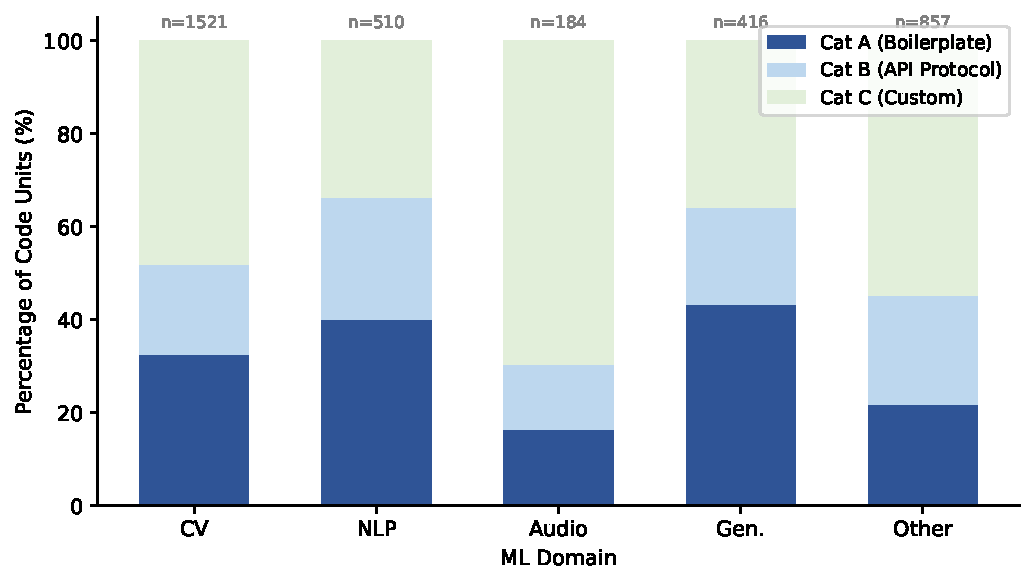
\includegraphics[width=0.85\textwidth]{figures/fig1_classification_by_domain.pdf}
\caption{Classification distribution by ML domain. Cat~A (framework boilerplate) and Cat~B (API protocol) together account for the majority of code units in most domains.}
\label{fig:classification_domain}
\end{figure}

\emph{Summary:} Across 15 projects, 31.4\% of code units were classified as Category~A (framework boilerplate), 21.2\% as Category~B (API protocol), and 47.3\% as Category~C (custom implementation). By lines of code, the proportions were 37.3\%, 18.4\%, and 44.3\% respectively. Combined, framework-dictated code (A+B) accounted for 52.7\% of all code units (55.7\% by LOC), meaning that only 47.3\% of code units in a typical PyTorch project represent custom developer work.

\subsection{RQ2: Baseline Similarity}

\begin{table}[t]
\centering
\caption{Pairwise similarity summary at standard threshold ($t=12$).}
\label{tab:similarity}
\small
\begin{tabular}{lrrrrr}
\toprule
Metric & Mean & Median & Q1 & Q3 & IQR \\
\midrule
Full-code similarity (\%) & 5.34 & 3.88 & 2.60 & 7.38 & 4.78 \\
Filtered similarity (\%) & 3.23 & 3.07 & 1.73 & 4.48 & 2.75 \\
Filtration effect (pp) & 2.11 & 1.17 & 0.15 & 3.97 & 3.82 \\
\midrule
Within-domain (\%) & 4.67 & & & & \\
Cross-domain (\%) & 5.55 & & & & \\
\bottomrule
\end{tabular}
\end{table}

\emph{Summary:} The mean pairwise similarity between independent projects using full code was 5.34\%, substantially above the $<$1\% baseline reported by Juergens et al.~\citep{juergens2010} for implementations without a shared framework. Within-domain pairs showed slightly lower similarity (4.67\%) than cross-domain pairs (5.55\%), though this difference was not statistically significant (Mann-Whitney $U = 977.5$, $p = 0.87$, Cliff's $\delta = -0.02$).

\subsection{RQ3: Filtration Effect}

\begin{table}[t]
\centering
\caption{Top 15 project pairs by filtration effect (standard threshold, $t=12$).}
\label{tab:filtration}
\small
\begin{tabular}{llrrrr}
\toprule
Project A & Project B & Full (\%) & Filt.\ (\%) & Effect (pp) & Red.\ (\%) \\
\midrule
Diff-Distill-WL & PyTorch-Ex & 15.35 & 6.42 & 8.94 & 58.2 \\
BenchmarkTL & Chatterbox-FT & 13.63 & 4.96 & 8.67 & 63.6 \\
ANTsTorch & Diff-Distill-WL & 11.83 & 3.33 & 8.49 & 71.8 \\
ANTsTorch & Chatterbox-FT & 11.75 & 3.28 & 8.47 & 72.1 \\
Chatterbox-FT & PyTorch-Ex & 12.23 & 4.18 & 8.05 & 65.8 \\
BenchmarkTL & TorchEBM & 11.47 & 3.46 & 8.01 & 69.8 \\
Chatterbox-FT & GFlowNet-Pep & 12.12 & 4.45 & 7.67 & 63.3 \\
Chatterbox-FT & TorchEBM & 9.52 & 1.91 & 7.61 & 79.9 \\
Diff-Distill-WL & Chatterbox-FT & 14.35 & 6.75 & 7.59 & 52.9 \\
LaneDet-UNet & PyTorch-Ex & 8.80 & 1.50 & 7.30 & 83.0 \\
ANTsTorch & BenchmarkTL & 10.83 & 3.54 & 7.29 & 67.3 \\
PyTorch-Ex & TrackNet & 13.22 & 5.95 & 7.27 & 55.0 \\
Diff-Distill-WL & GFlowNet-Pep & 10.51 & 3.34 & 7.17 & 68.2 \\
Diff-Distill-WL & TorchEBM & 8.24 & 1.39 & 6.85 & 83.1 \\
LaneDet-UNet & TrackNet & 9.87 & 3.07 & 6.81 & 69.0 \\
\bottomrule
\end{tabular}
\end{table}

\begin{figure}[t]
\centering
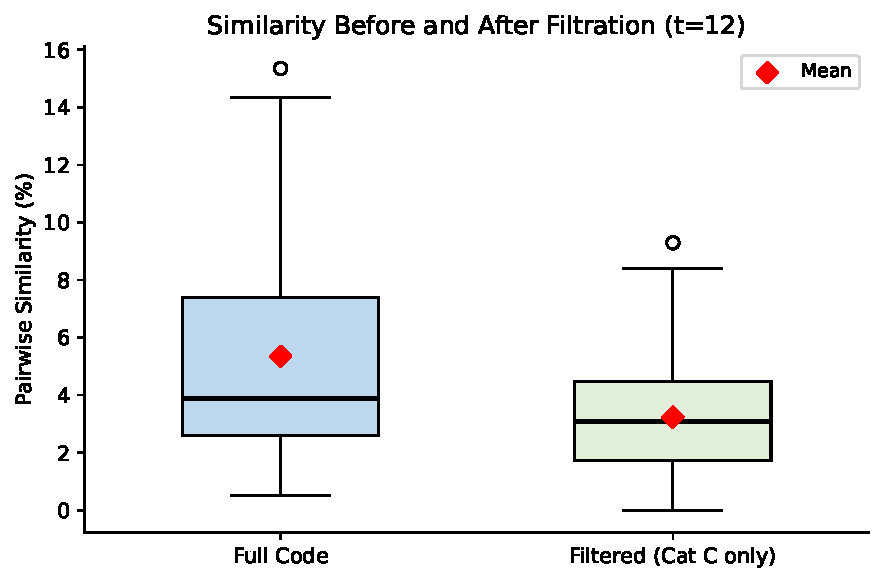
\includegraphics[width=0.7\textwidth]{figures/fig2_boxplot_filtration.pdf}
\caption{Distribution of pairwise similarity before (full code) and after (filtered, Category~C only) removing framework-dictated code. Red diamonds indicate means.}
\label{fig:boxplot_filtration}
\end{figure}

\emph{Summary:} Filtering framework boilerplate reduced mean pairwise similarity from 5.34\% to 3.23\%, a reduction of 2.11 percentage points (39.5\% relative reduction). The filtration effect was statistically significant (Wilcoxon signed-rank $W = 914$, $p < 0.001$, Cliff's $\delta = 0.33$), with 76.2\% of pairs showing a positive filtration effect. This demonstrates that a substantial portion of measured similarity between independent PyTorch projects is attributable to shared framework code rather than meaningful design similarity.

\subsection{RQ4: Sensitivity Analysis}

\begin{figure}[t]
\centering
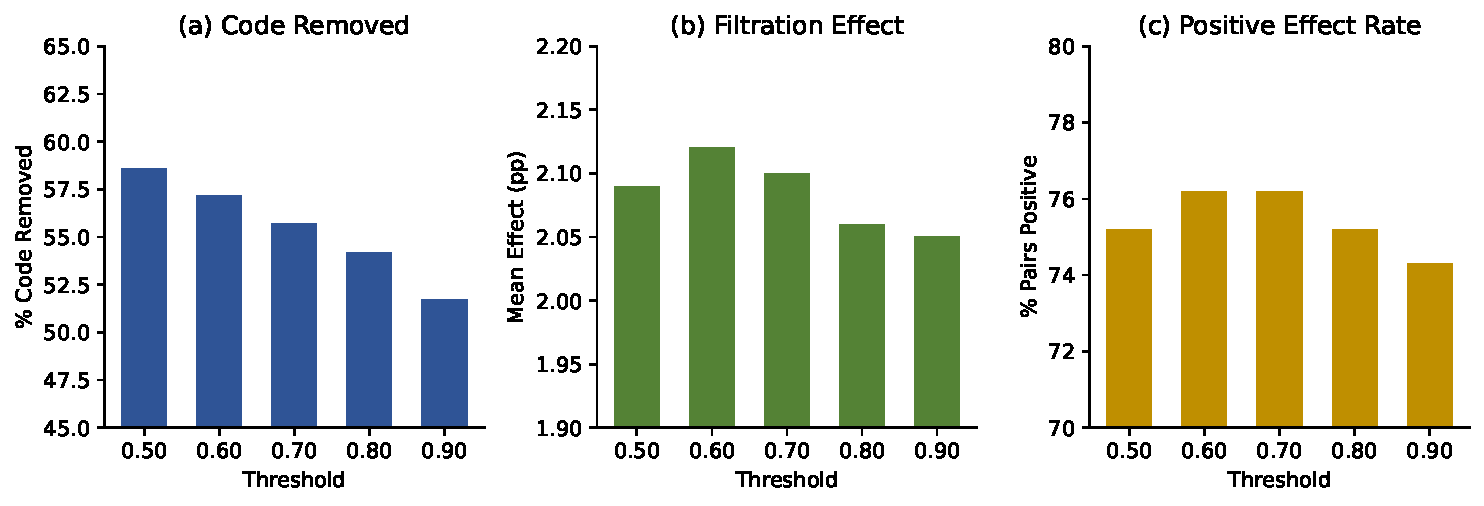
\includegraphics[width=\textwidth]{figures/fig3_sensitivity.pdf}
\caption{Sensitivity of key metrics to classification threshold. (a)~Percentage of code removed. (b)~Mean filtration effect in percentage points. (c)~Percentage of pairs with positive filtration effect. All metrics are stable across the 0.50--0.90 range.}
\label{fig:sensitivity}
\end{figure}

\begin{table}[t]
\centering
\caption{Core findings at each classification threshold (JPlag $t=12$).}
\label{tab:sensitivity}
\small
\begin{tabular}{rrrrrr}
\toprule
Threshold & Code Rem.\ (\%) & Mean Full (\%) & Mean Filt.\ (\%) & Effect (pp) & Pos.\ Effect (\%) \\
\midrule
0.50 & 58.6 & 5.34 & 3.26 & 2.09 & 75.2 \\
0.60 & 57.2 & 5.34 & 3.23 & 2.12 & 76.2 \\
0.70 & 55.7 & 5.33 & 3.23 & 2.10 & 76.2 \\
0.80 & 54.2 & 5.35 & 3.29 & 2.06 & 75.2 \\
0.90 & 51.7 & 5.33 & 3.29 & 2.05 & 74.3 \\
\bottomrule
\end{tabular}
\end{table}

\emph{Summary:} The boilerplate proportion (A+B as percentage of code removed) varied by only 6.9 percentage points across the five classification thresholds tested (range: 51.7--58.6\%). The filtration effect was similarly stable, varying by only 0.07 percentage points (range: 2.05--2.12pp). This stability indicates that the core findings are robust to the specific classification threshold chosen.


% ============================================================
\section{Discussion}
\label{sec:discussion}

\subsection{Key Findings}

The central finding of this study is that a majority of code in independent PyTorch projects is framework-dictated. At the default classification threshold, 52.7\% of code units (A+B combined) represent boilerplate or API protocol code. This means that code similarity tools, when applied to PyTorch projects without filtering, are primarily measuring framework conformity rather than developer-specific design decisions.

The filtration effect (the reduction in measured similarity after removing framework code) confirms this interpretation quantitatively. The 2.11-percentage-point reduction from full-code to custom-only similarity (a 39.5\% relative reduction) demonstrates that a substantial portion of detected ``similarity'' between independent projects is an artifact of shared framework constraints.

\subsection{Comparison with Prior Work}

Juergens et al.~\citep{juergens2010} reported $<$1\% clone detection rates for 109 independent implementations of the same specification without a shared framework. Our results show that when a shared framework is introduced, baseline similarity increases to 5.34\%, more than five times higher. This confirms the hypothesis that framework constraints fundamentally change the interpretation of code similarity measurements.

Sens et al.~\citep{sens2025} found 58\% duplication in ML systems. Our measurements suggest that a large portion of this duplication may be framework-dictated rather than representing meaningful code reuse. The 52.7\% boilerplate proportion we measured provides context for interpreting their finding.

\subsection{Implications for Practice}

These findings have direct implications for any setting where code similarity scores are used to draw conclusions about ML software:

\emph{Clone detection research.} Studies measuring clone rates in ML code should account for framework boilerplate to avoid inflating reported rates. Our classifier and filtering methodology provide a reusable tool for this purpose.

\emph{Plagiarism detection.} In educational settings where students submit PyTorch assignments, similarity tools will report high baseline scores between independent submissions. Instructors should calibrate expectations against the baselines reported here.

\emph{Forensic software analysis.} In intellectual property disputes involving ML software, similarity scores must be interpreted in light of the framework effect. A similarity score that falls within the range of framework-driven coincidence documented here is qualitatively different from one that exceeds it.

\subsection{Limitations of the Filtration Effect}

The filtration effect as measured here is a \emph{lower bound} on the true framework contribution to similarity. Our binary filtering (remove A+B, keep C) may not capture all framework influence; some Category~C code may still be indirectly shaped by framework conventions (e.g., tensor shape conventions that propagate into custom code). Additionally, our Category~B (API protocol) code occupies a gray area: it follows framework patterns but includes domain-specific content.


% ============================================================
\section{Threats to Validity}
\label{sec:threats}

\subsection{Construct Validity}

The primary construct validity concern is the accuracy of the AST-based classifier. The three-category classification scheme necessarily involves boundary cases, particularly for \texttt{nn.Module} subclasses that contain both framework-dictated structure and custom logic. We address this through: (1)~validation against PyTorch documentation as objective ground truth, (2)~a detailed codebook with explicit boundary-case rules, and (3)~sensitivity analysis showing that findings are stable across thresholds.

The choice of JPlag (token-based) over NiCad (AST-based) for similarity measurement means our results capture syntactic rather than structural similarity. Token-based comparison is arguably more conservative, which would make positive findings about accidental clones more robust. However, results may differ with AST-based tools, and we identify cross-tool comparison as future work.

\subsection{Internal Validity}

The study uses a solo-researcher validation design. Intra-rater reliability measures classification consistency but not objectivity; the same systematic bias could affect both rounds. A multi-rater validation study with independent software engineers would strengthen construct validity. We plan this as a follow-up study and acknowledge it as an explicit limitation.

\subsection{External Validity}

Our study examines a single framework (PyTorch) in a single language (Python) across a limited number of projects (15). While PyTorch is the most widely used ML research framework, results may not generalize to TensorFlow, JAX, or frameworks in other languages. The specific project selection criteria (500--5{,}000 LOC, $\leq$3 contributors, 30+ commits) target a particular project profile; larger or more complex projects may exhibit different boilerplate proportions.

We focus on five ML domains (computer vision, NLP, audio, generative modeling, and other). Additional domains (reinforcement learning, graph neural networks) may have different framework usage patterns.

\subsection{Conclusion Validity}

The small sample size (15 projects, 105 pairwise comparisons) limits statistical power. We use non-parametric tests appropriate for small samples and report effect sizes alongside $p$-values. Bootstrap confidence intervals provide uncertainty quantification. We frame this as an initial measurement study; larger replications are future work.


% ============================================================
\section{Conclusion and Future Work}
\label{sec:conclusion}

This paper presents the first empirical measurement of framework-driven code similarity in ML software. Across 15 independent PyTorch projects, we found that 52.7\% of code units are classifiable as framework boilerplate or API protocol code, leaving only 47.3\% as custom implementation. Filtering framework code reduced measured pairwise similarity by 2.11 percentage points (39.5\% relative reduction), demonstrating that a substantial portion of detected similarity between independent ML projects is an artifact of shared framework constraints rather than meaningful design similarity. These findings were stable across five classification thresholds (filtration effect range: 0.07 percentage points).

These baselines have immediate practical value for clone detection research, plagiarism detection in educational settings, and forensic software analysis involving ML code. A similarity score between two PyTorch projects that falls within the framework-driven range documented here should not be interpreted as evidence of copying.

\subsection{Future Work}

Several directions for extension are planned. First, expanding to TensorFlow and Hugging Face Transformers would test whether the framework effect generalizes across ML ecosystems. Second, a larger dataset (50+ projects) with multi-rater validation would strengthen both statistical power and construct validity. Third, semantic similarity tools such as CodeBERT could complement token-based comparison to capture Type-4 clones. Fourth, a dedicated forensic methodology paper would apply these baselines to propose calibrated interpretation guidelines for ML software IP disputes.

\subsection{Replication Package}

All data, code, and analysis scripts are available at \placeholder{Zenodo DOI URL}. The package includes: the AST classifier source code, classification manifests for all projects, the intra-rater validation data and codebook, JPlag configuration and results, sensitivity analysis notebooks, and pre-generated tables and figures.


% ============================================================
% References
% ============================================================
\bibliographystyle{plainnat}

\begin{thebibliography}{99}

\bibitem[Ain et~al.(2019)]{ain2019}
Ain, Q.U., Butt, W.H., Anwar, M.W., Azam, F., \& Maqbool, B. (2019).
\newblock A systematic review on code clone detection.
\newblock \emph{IEEE Access}, 7, 86121--86144.

\bibitem[Cordy \& Roy(2011)]{cordy2011}
Cordy, J.R. \& Roy, C.K. (2011).
\newblock The {NiCad} clone detector.
\newblock In \emph{Proc.\ 19th Int.\ Conf.\ on Program Comprehension (ICPC)}, pp.\ 219--220.

\bibitem[Juergens et~al.(2010)]{juergens2010}
Juergens, E., Deissenboeck, F., \& Hummel, B. (2010).
\newblock Code similarities beyond copy \& paste.
\newblock In \emph{Proc.\ 14th European Conf.\ on Software Maintenance and Reengineering (CSMR)}, pp.\ 78--87.

\bibitem[Kapser \& Godfrey(2008)]{kapser2008}
Kapser, C.J. \& Godfrey, M.W. (2008).
\newblock ``{Cloning Considered Harmful}'' considered harmful: Patterns of cloning in software.
\newblock \emph{Empirical Software Engineering}, 13(6), 645--692.

\bibitem[Nahar et~al.(2025)]{nahar2025}
Nahar, N., et~al. (2025).
\newblock A meta-summary of challenges in building products with {ML} components.
\newblock In \emph{Proc.\ 47th Int.\ Conf.\ on Software Engineering (ICSE)}.

\bibitem[Prechelt et~al.(2000)]{jplag2000}
Prechelt, L., Malpohl, G., \& Philippsen, M. (2000).
\newblock {JPlag}: Finding plagiarisms among a set of programs.
\newblock Technical Report 2000-1, Universit\"{a}t Karlsruhe.

\bibitem[Ragkhitwetsagul et~al.(2018)]{ragkhitwetsagul2018}
Ragkhitwetsagul, C., Krinke, J., \& Clark, D. (2018).
\newblock A comparison of code similarity analysers.
\newblock \emph{Empirical Software Engineering}, 23(4), 2464--2519.

\bibitem[Roy \& Cordy(2007)]{roy2007survey}
Roy, C.K. \& Cordy, J.R. (2007).
\newblock A survey on software clone detection research.
\newblock Technical Report 2007-541, Queen's University, School of Computing.

\bibitem[Roy et~al.(2009)]{roy2009}
Roy, C.K., Cordy, J.R., \& Koschke, R. (2009).
\newblock Comparison and evaluation of code clone detection techniques and tools: A qualitative approach.
\newblock \emph{Science of Computer Programming}, 74(7), 470--495.

\bibitem[Sens et~al.(2025)]{sens2025}
Sens, Y., et~al. (2025).
\newblock A large-scale study of model integration in {ML}-enabled software systems.
\newblock In \emph{Proc.\ 47th Int.\ Conf.\ on Software Engineering (ICSE)}.

\bibitem[Svajlenko \& Roy(2015)]{svajlenko2015}
Svajlenko, J. \& Roy, C.K. (2015).
\newblock Evaluating clone detection tools with {BigCloneBench}.
\newblock In \emph{Proc.\ Int.\ Conf.\ on Software Maintenance and Evolution (ICSME)}, pp.\ 131--140.

\end{thebibliography}

\end{document}
